\chapter{Analyse du problème}
\setcounter{minitocdepth}{2}
\minitoc

\section{Introduction}
L'objectif du premier livrable est d'analyser la méthode GTD afin de pouvoir par la suite en développer un outil. Dans notre cas, il s'agira d'un client permettant l'exploitation de cette méthode. Nous devons pour cela identifier les différents cas d'utilisation, et les décrire à l'aide du canevas de Cockburn, ainsi qu'à l'aide des différents outils UML tels les diagrammes de séquences, de classes, etc.

\section{Dictionnaire de données}
Afin que les termes employés soient correctement interprétés par tous, nous les avons définis dans un dictionnaire de données.

\begin{tabular}{|p{1.7cm}|p{6cm}|p{1.7cm}|p{1.7cm}|}
\hline
\textbf{Notion} & \textbf{Définition} & \textbf{Traduit en...} & \textbf{Nom informatique} \\
\hline
Chose à faire & Toute idée, pensée, activité pouvant nécessiter une action de la part de l'\textbf{utilisateur} et devant être renseignée par la suite & & \\
\hline
Contact & Ensemble d'attributs (nom, numéro de téléphone, email, etc.) définissant un contact & Classe & Contact \\
\hline
Contexte & L'endroit où l'on se trouve, les outils disponibles, les limites et possibilités de l'environnement & Classe & Contexte \\
\hline
Echéance & Date butoir jusqu'à laquelle la \textbf{tâche} peut être accomplie & & \\
\hline
Fréquence de répétition & La fréquence à laquelle se répète la \textbf{tâche} (journalière, mensuelle, etc.) & & \\
\hline
Priorité & Valeur comprise entre 1 et 5 traduisant l'urgence de la \textbf{tâche} & & \\
\hline
Projet & Ensemble de \textbf{tâches} et de sous-projets, ayant une finalité propre et définissant un \textbf{contexte} par défaut & Classe & Projet \\
\hline
Tâche & Action atomique, pouvant être contenue dans un \textbf{projet}, et pouvant contenir un nom, une date de début, une \textbf{échéance}, des notes, une \textbf{priorité}, un \textbf{taux d'effort demandé}, une liste de \textbf{contacts}, une \textbf{fréquence de répétition}, une date d'arrêt de la répétition, des liens, des \textbf{tags} & Classe & Tache \\
\hline
Tags & Mots-clés liés à une \textbf{tâche} & & \\
\hline
Taux d'effort demandé & Valeur comprise entre 0 et 99 définissant la complexité supposé de la \textbf{tâche} & & \\
\hline
Utilisateur & Toute personne ayant recours à la méthode GTD & Acteur & User \\
\hline
\end{tabular}
\newpage
\begin{tabular}{|p{1.7cm}|p{6cm}|p{1.7cm}|p{1.7cm}|}
\hline
\textbf{Action} & \textbf{Définition} & \textbf{Traduit en...} & \textbf{Nom informatique} \\
\hline
Collecter & Action qui permet de recenser toutes les \textbf{choses à faire} à traiter & Opération & Collect \\
\hline
Examiner & Action de mise à jour du système GTD & Opération & Review \\
\hline
Faire & Choix de la \textbf{tâche} à effectuer immédiatement & Opération & Do \\
\hline
Organiser & Action de classement des \textbf{tâches} par rapport à leurs attributs (\textbf{priorité}, \textbf{échéance}, etc.) & Opération & Organize \\
\hline
Spécifier une chose à faire & Spécifier la tâche correspondant à la chose à faire ou en faire un projet (ou sous-projet) & Opération & Specify \\
\hline
Traiter & Action de renseignement des tâches collectées & Opération & Process \\
\hline
\end{tabular}


\section{Cas d'utilisation}

Après une recherche approfondie sur la méthode GTD, nous avons retenu cinq cas majeurs d'utilisation~:
\begin{enumerate}
\item Collecter des choses à faire.
\item Traiter ces choses à faire.
\item Organiser les tâches issues du traitement.
\item Examiner régulièrement ces tâches et ajouter celles en attente.
\item Sélectionner une tâche afin de la réaliser.
\end{enumerate}

Nous obtenons alors le diagramme de cas d'utilisation de la figure \ref{usecase}.

\begin{figure}[!ht]
\begin{center}
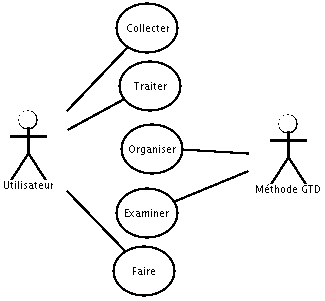
\includegraphics[width=7cm]{images/usecase.png}
\caption{Diagramme de cas d'utilisation}
\label{usecase}
\end{center}
\end{figure}

%%%%%%%%% USE CASE 1 %%%%%%%%%

\subsection{Collecter les informations}
L'objectif de ce cas d'utilisation est de recenser tout ce à quoi on pense et qu'on peut être amené à réaliser par la suite. Ces idées doivent pouvoir être notées rapidement, car elles peuvent apparaître à un moment où l'on est occupé (au téléphone, en réunion, etc.).

\subsubsection{Canevas de Cockburn}

\begin{usecase}{Collecter des choses à faire}
\begin{information}
\item[Goal in context~:] Récupérer des choses à faire et les ajouter à la liste de choses à faire
\item[Scope~:] La méthode GTD
\item[Level~:] Summary
\item[Pre-conditions~:] Avoir des choses à faire non classées dans GTD
\item[Post-conditions~:] Aucune chose à faire perdue
\item[Success End Condition~:] Toutes les choses à faire voulues ont été rentrées
\item[Failed End Condition~:] Les choses à faire données par l'utilisateur ont été perdues
\item[Primary actor~:] L'utilisateur, toute personne voulant être mieux organisée
\item[Trigger~:] L'utilisateur a demandé à rentrer des choses à faire
\\
\end{information}
\begin{scenario}
\item L'utilisateur demande à ajouter des choses à faire
\item La méthode GTD enregistre les choses à faire
\item L'utilisateur arrête la saisie
\\
\end{scenario}
\begin{relatedinformation}
\item[Priority~:] Faible
\item[Performance target~:] Quelques secondes par chose à faire
\item[Frequency~:] Régulièrement (potentiellement tous les jours)
\item[Channel to primary actor~:] Action directe de l'utilisateur
\\
\end{relatedinformation}
\begin{openissues}
\item Que se passe-t-il si le système perd une ou plusieurs choses à faire~?
\\
\end{openissues}
\end{usecase}

\subsubsection{Instantané}
Avant application de ce cas d'utilisation (figure \ref{collect1}), on obtient une liste des choses à faire auquelles on a ajouté des éléments (figure \ref{collect2}).

\begin{figure}[!ht]
\begin{center}
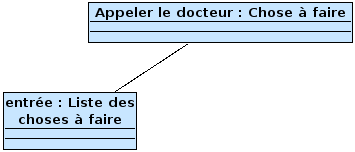
\includegraphics[width=6cm]{images/Instantane_Collect_1.png}
\caption{Etat du système \emph{avant} la collecte}
\label{collect1}
\end{center}
\end{figure}

\begin{figure}[!ht]
\begin{center}
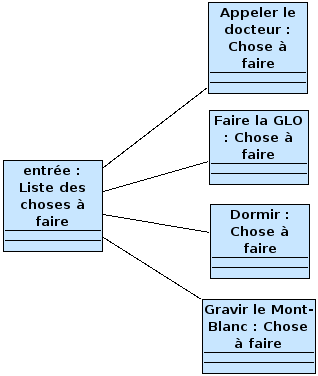
\includegraphics[width=6cm]{images/Instantane_Collect_2.png}
\caption{Etat du système \emph{après} la collecte}
\label{collect2}
\end{center}
\end{figure}

\subsubsection{Contraintes OCL}

Nous n'avons pas défini de contraintes OCL pour ce cas d'utilisation.

\subsubsection{Diagramme de séquence}
figure \ref{collectSequence}.
\begin{figure}[!ht]
\begin{center}
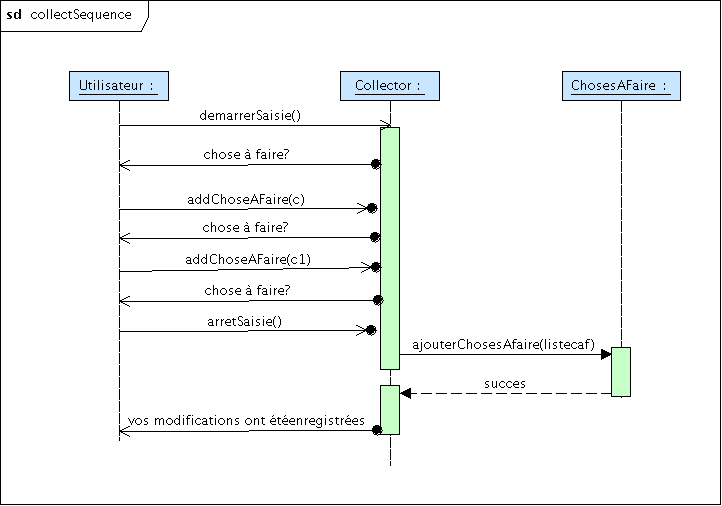
\includegraphics[width=12cm]{images/collectSequence.png}
\caption{Scénario de collecte des choses à faire}
\label{collectSequence}
\end{center}
\end{figure}


%%%%%%%%% USE CASE 2 %%%%%%%%%

\subsection{Traiter ces informations}
Après la collecte des informations, il faut leur appliquer un traitement afin connaître certaines propriétés essentielles pour le système, telles le contexte de la tâche, la périodicité, l'échéance, etc.

\subsubsection{Canevas de Cockburn}

\begin{usecase}{Collecter des choses à faire}
\begin{information}
\item[Goal in context~:] On effectue le traitement (création d'un projet contenant une décomposition de la tâche courante, ordonner à l'utilisateur de faire la tâche, la déléguer, la reporter, l'archiver) d'une ou plusieurs choses à faire de la liste
\item[Scope~:] La gestion des priorités après traitement, la création de la liste de choses à faire
\item[Level~:] Summary
\item[Pre-conditions~:] Liste de choses à faire non-vide
\item[Post-conditions~:] Les tâches traitées apparaissent dans les donnée stockée
\item[Success End Condition~:] Le chose à faire supprimée de la liste a été traitée
\item[Failed End Condition~:] Le traitement a échoué
\item[Primary actor~:] L'utilisateur
\item[Trigger~:] L'utilisateur
\\
\end{information}
\begin{scenario}
\item L'utilisateur demande à lancer le traitement des éléments de la liste des choses à faire
\item La méthode GTD émet une demande de renseignements des attributs de la chose à faire, en vue d'en faire une tâche
\item L'utilisateur rentre ou non des informations
\item La méthode GTD applique le traitement à la tâche ou le projet
\item La méthode GTD supprime la chose à faire qui vient d'être traitée
\item Arrêt de la procédure de traitement
\\
\end{scenario}
\begin{variation}
\item[3a] L'utilisateur rentre ou non des informations
\item[3a1] L'utilisateur effectue la tâche immédiatement et retour à l'étape 2.
\item[3a2] Il n'y a pas encore de contexte adapté à cette tâche, création d'un nouveau contexte.
\item[6a] L'utilisateur rentre ou non des informations et demande la chose à faire suivante
\item[6a1] On remplace l'arrêt du traitement par le retour à l'étape 2.
\\
\end{variation}
\begin{relatedinformation}
\item[Priority~:] Moyenne
\item[Performance target~:] Moins de deux minutes
\item[Frequency~:] Régulièrement (une fois par semaine)
\item[Channel to primary actor~:] Action directement effectuée par l'utilisateur
\\
\end{relatedinformation}
\begin{openissues}
\item Que se passe-t-il si la chose à faire n'est pas sauvegardée~?
\item Que se passe-t-il si la chose à faire n'est pas supprimée~?
\\
\end{openissues}
\end{usecase}

\subsubsection{Instantané}

Après traitement de données du système (figure \ref{process1}), des tâches sont créés et associées à des contextes (figure \ref{process2}).

\begin{figure}[!ht]
\begin{center}
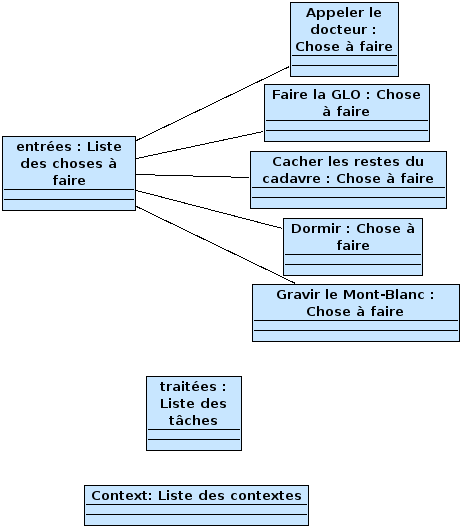
\includegraphics[width=10cm]{images/Instantane_Process_1.png}
\caption{Etat du système \emph{avant} le traitement}
\label{process1}
\end{center}
\end{figure}

\begin{figure}[!ht]
\begin{center}
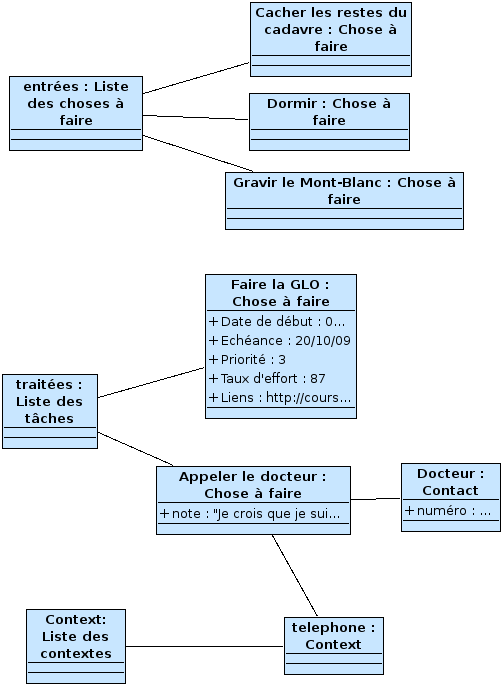
\includegraphics[width=10cm]{images/Instantane_Process_2.png}
\caption{Etat du système \emph{après} le traitement}
\label{process2}
\end{center}
\end{figure}

\subsubsection{Contraintes OCL}

\begin{ocl}
-- La taille de liste de choses a faire doit etre decrementee,
-- et au moins un conteneur de taches doit posseder des
-- elements supplementaires
context Traitement::traiterChoseAFaire()
pre Collector.getListeChoseAFaire().size() > 0
post Collector.getListeChoseAFaire().size()@pre >
		Collector.getListeChoseAFaire().size()
	and (NextAction.size() > NextAction.size()@pre
	or WaitFor.size() > WaitFor.size()@pre
	or Someday.size() > Someday.size()@pre
	or Archive.size() > Archive.size()@pre)
\end{ocl}

\subsubsection{Diagramme de séquence}
Dans le cas où la chose à faire correspond à une simple tâche, nous obtenons le diagramme de séquence de la figure \ref{traitementSequence}.
\begin{figure}[!ht]
\begin{center}
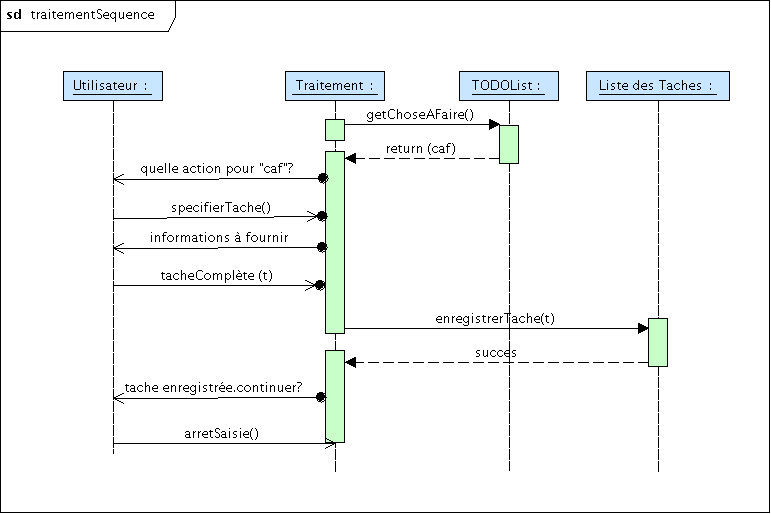
\includegraphics[width=12cm]{images/traitementSequence.png}
\caption{Scénario de traitement d'une chose à faire}
\label{traitementSequence}
\end{center}
\end{figure}

%%%%%%%%% USE CASE 3 %%%%%%%%%

\subsection{Organiser les tâches issues du traitement}

\subsubsection{Canevas de Cockburn}

\begin{usecase}{Organiser les éléments stockés dans les dossiers}
\begin{information}
\item[Goal in context~:] Gérer les priorités, les contextes et tout autres attributs pour définir l'ensemble des prochaines actions à partir des tâches dans les dossier.
\item[Scope~:] La création des tâches, leurs actions et leurs attributs.
\item[Level~:] Primary Task
\item[Pre-conditions~:] /
\item[Post-conditions~:] /
\item[Success End Condition~:] Toutes les tâches ont été triées.
\item[Failed End Condition~:] Tâches inorganisable, erreur système.
\item[Primary actor~:] Le système
\item[Trigger~:] Après le traitement/Après chaque modification
\\
\end{information}
\begin{scenario}
\item Le système requiert de l'ordre
\item Les éléments mal-placés ou entrants sont déplacés au bon endroit
\\
\end{scenario}
\begin{relatedinformation}
\item[Priority~:] Haute
\item[Performance target~:] Invisible à l'utilisateur
\item[Frequency~:] Après le traitement/Après chaque modification
\\
\end{relatedinformation}
\begin{openissues}
\item Que se passe-t-il dans le cas de conflit priorité/échéance ?
\\
\end{openissues}
\end{usecase}


\subsubsection{Instantané}

Avant organisation (figure \ref{organize1}), nous avons une liste de tâches dont les éléments se font spécifier (figure \ref{organize2}).

\begin{figure}[!ht]
\begin{center}
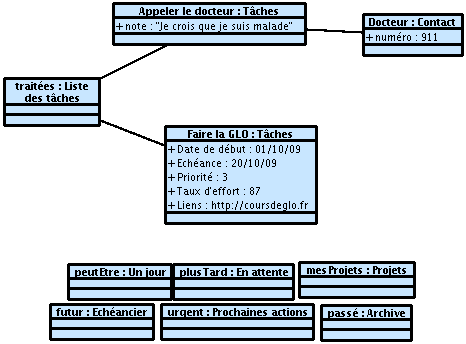
\includegraphics[width=10cm]{images/Instantane_Organize_1.png}
\caption{Etat du système \emph{avant} l'organisation}
\label{organize1}
\end{center}
\end{figure}

\begin{figure}[!ht]
\begin{center}
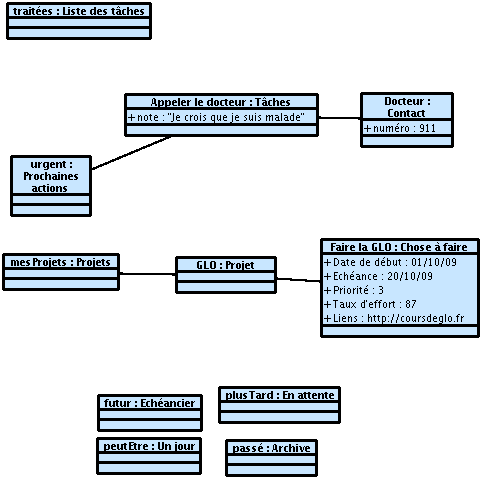
\includegraphics[width=10cm]{images/Instantane_Organize_2.png}
\caption{Etat du système \emph{après} l'organisation}
\label{organize2}
\end{center}
\end{figure}

\subsubsection{Contraintes OCL}

Nous n'avons pas défini de contraintes OCL pour ce cas d'utilisation.

\subsubsection{Diagramme de séquence}
Le scénario de l'organisation des tâches est décris par la figure \ref{organizeSequence}.
\begin{figure}[!ht]
\begin{center}
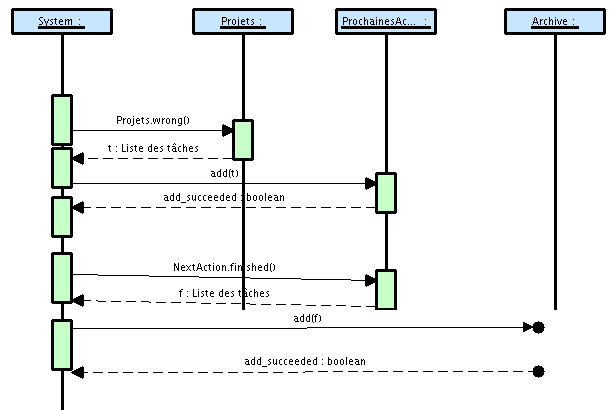
\includegraphics[width=12cm]{images/organizeSequence.png}
\caption{Scénario d'organisation des tâches}
\label{organizeSequence}
\end{center}
\end{figure}


%%%%%%%%% USE CASE 4 %%%%%%%%%

\subsection{Examiner régulièrement ces tâches et ajouter celles en attente}

\subsubsection{Canevas de Cockburn}

\begin{usecase}{Vérification des données stockées}
\begin{information}
\item[Goal in context~:] Vérifier si aucune tâche dans En Attente ou dans Un Jour n'est passée à l'état actif  et met l'échéancier à jour..
\item[Scope~:] Les tâches
\item[Level~:] Primary Task
\item[Pre-conditions~:] Il y a des tâches à examiner.
\item[Post-conditions~:] L'échéancier a été mis à jour.
\item[Success End Condition~:] Toutes les tâches examinées ont été activées
\item[Failed End Condition~:] Erreur système.
\item[Primary actor~:] Le système
\item[Trigger~:] Automatique
\\
\end{information}
\begin{scenario}
\item Vérifier dans En Attente si des tâches sont devenues actives
\item Vérifier dans Un Jour si il est possible de réaliser une tâche
\item Vérification si il y a un jour1 dans l'échéancier, et, si c'est le cas, ajoute ses projets dans le dossier Projets (en ajoutant sa première tâche dans Prochaines Actions) .
\item Mettre à jour l'échéancier
\item Transférer les tâches dans Prochaines Action
\\
\end{scenario}
\begin{relatedinformation}
\item[Priority~:] Haute
\item[Frequency~:] Une fois par jour
\\
\end{relatedinformation}
\end{usecase}

\subsubsection{Instantané}

Avant l'examen des tâches (figure \ref{review1}), nous avons une organisation qui va être remaniée par cette opération (figure \ref{review2}).

\begin{figure}[!ht]
\begin{center}
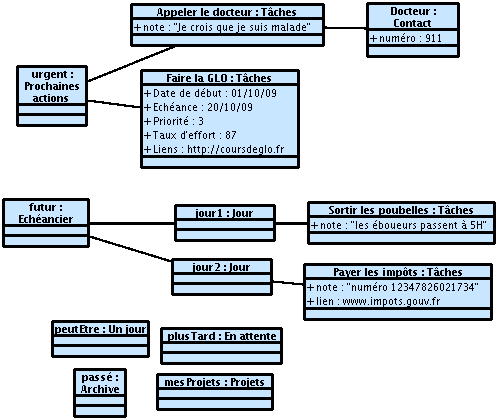
\includegraphics[width=10cm]{images/Instantane_Review_1.png}
\caption{Etat du système \emph{avant} la mise à jour des tâches de l'échéancier}
\label{review1}
\end{center}
\end{figure}

\begin{figure}[!ht]
\begin{center}
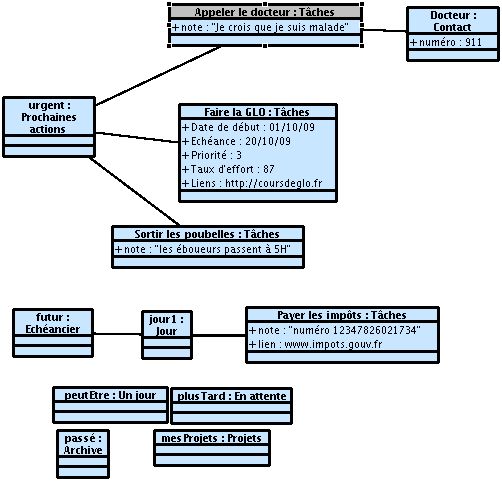
\includegraphics[width=10cm]{images/Instantane_Review_2.png}
\caption{Etat du système \emph{après} la mise à jour des tâches de l'échéancier}
\label{review2}
\end{center}
\end{figure}

\subsubsection{Contraintes OCL}

\begin{ocl}
-- Il doit au moins y avoir une tache a examiner
context Examen::review())
pre WaitFor.size() > 0
	or Someday.size() > 0
	or Echeancier.size() > 0
post Echeancier.jour1.getEcheance() = Date.today()
\end{ocl}

\subsubsection{Diagramme de séquence}
Le scénario type de ce cas d'utilisation est décris par la figure \ref{reviewSequence}.
\begin{figure}[!ht]
\begin{center}
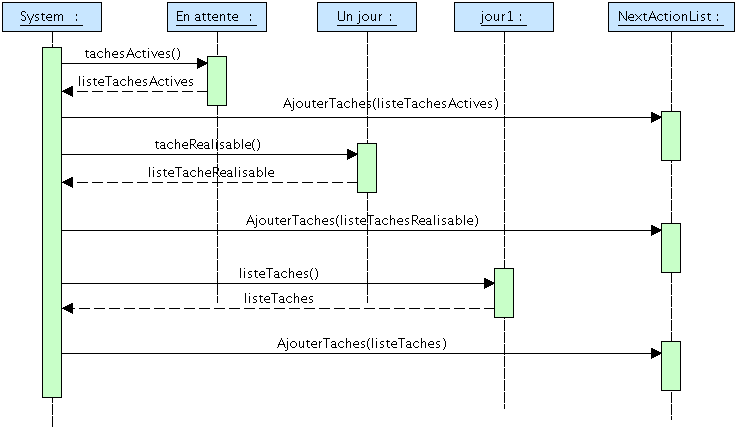
\includegraphics[width=12cm]{images/reviewSequence.png}
\caption{Scénario du cas d'utilisation examen}
\label{reviewSequence}
\end{center}
\end{figure}

%%%%%%%%% USE CASE 5 %%%%%%%%%

\subsection{Sélectionner une tâche afin de la réaliser}

\subsubsection{Canevas de Cockburn}

\begin{usecase}{Réaliser une tâche}
\begin{information}
\item[Goal in context~:] Obliger l'utilisateur à effectuer la tâche la plus prioritaire dans le dossier Prochaines Actions dans son contexte.
\item[Scope~:] Le contenu des Prochaines Actions
\item[Level~:] PrimaryTask
\item[Pre-conditions~:] L'utilisateur a du temps pour réaliser une tâche et il y a des tâches à effectuer.
\item[Post-conditions~:] L'utilisateur à réalisée la tâche prédéfini.
\item[Success End Condition~:] Ancienne tâche archivée et la seconde Prochaine Action devient la première.
\item[Failed End Condition~:] La tâche n'a pas été supprimée ou l'utilisateur n'a pas réalisé son travail.
\item[Primary actor~:] L'utilisateur
\item[Trigger~:] L'utilisateur
\\
\end{information}
\begin{scenario}
\item L'utilisateur demande à faire une tâche
\item L'utilisateur donne le contexte dans lequel il se trouve.
\item La méthode GTD choisit la tâche.
\item L'utilisateur indique qu'il a fini la tâche
\item La tâche est supprimée
\item Mise à jour des Prochaines Actions
\item L'utilisateur ne fait plus d'actions
\\
\end{scenario}
\begin{extension}
\item[4a] L'utilisateur n'a pas fini la tâche.
\item[4a1] La méthode GTD ne modifie rien.
\item[7a] L'utilisateur demande une nouvelle tâche à faire
\item[7a1] Retour à l'étape 3.
\\
\end{extension}
\begin{variation}
\item[6.1] Si une tâche est En Attente de la tâche réalisée, le système doit en informer l'utilisateur comme Prochaine Action à réaliser.
\\
\end{variation}
\begin{relatedinformation}
\item[Priority~:] Haute
\item[Frequency~:] Le plus souvent possible
\\
\end{relatedinformation}
\begin{openissues}
\item Que se passe-t-il si l'utilisateur ne finit jamais de tâches~?
\\
\end{openissues}
\end{usecase}

\subsubsection{Instantané}

Avant la réalisation de la tâche (figure \ref{do1}), la prochaine tâche devant être exécuté est (dans notre exemple) d'appeler un docteur. Cette tâche est alors désignée pour être terminée (figure \ref{do2}).

\begin{figure}[!ht]
\begin{center}
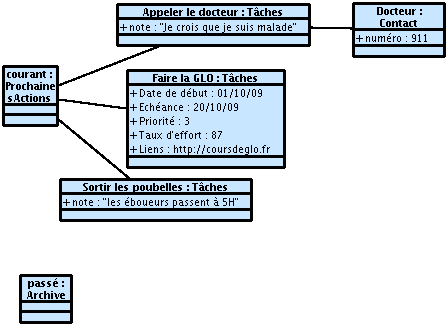
\includegraphics[width=10cm]{images/Instantane_Do_1.png}
\caption{Etat du système \emph{avant} la réalisation d'une tâche}
\label{do1}
\end{center}
\end{figure}

\begin{figure}[!ht]
\begin{center}
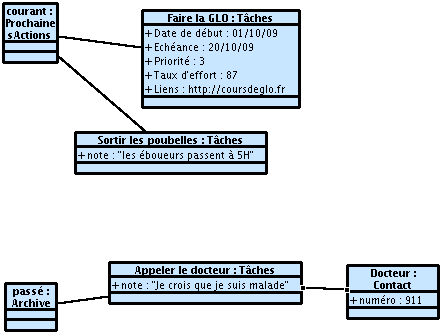
\includegraphics[width=10cm]{images/Instantane_Do_2.png}
\caption{Etat du système \emph{après} la réalisation d'une tâche}
\label{do2}
\end{center}
\end{figure}

\subsubsection{Contraintes OCL}

\begin{ocl}
-- Une fois la tache "NextAction" accomplie, celle qui etait
-- en deuxieme sur la liste des actions devient la
-- nouvelle "NextAction"
context Do::do()
pre NextAction.size() > 0
post NextAction.second()@pre = NextAction.first()
\end{ocl}

\subsubsection{Diagramme de séquence}
Le scénario de la réalisation d'une tâche est décrit par la figure \ref{doSequence}.
\begin{figure}[!ht]
\begin{center}
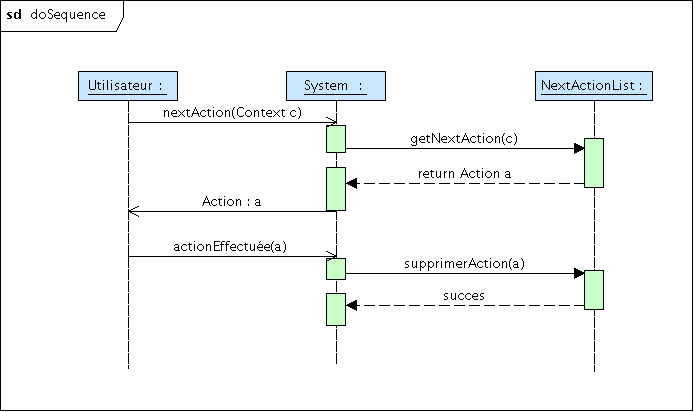
\includegraphics[width=12cm]{images/doSequence.png}
\caption{Scénario de réalisation d'une tâche}
\label{doSequence}
\end{center}
\end{figure}

\chapter{Analyse finale}

L'analyse de tous les cas d'utilisation du système nous a permis de concevoir le diagramme de classe de la figure \ref{ddc}.

\begin{figure}[!ht]
\begin{center}
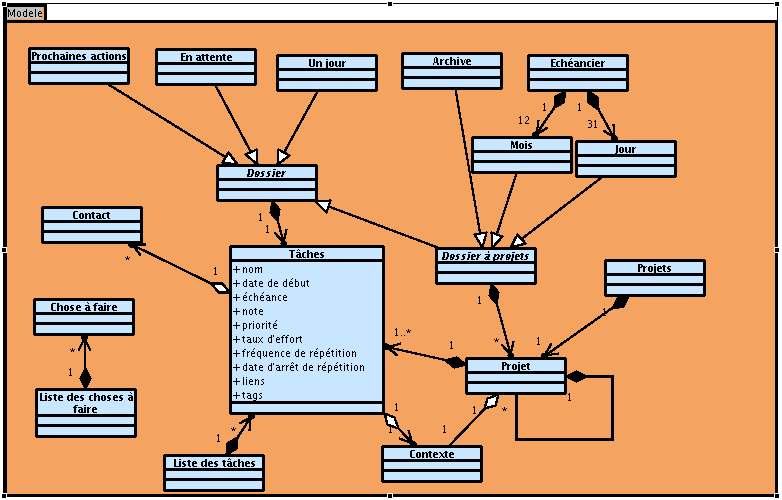
\includegraphics[width=12cm]{images/DiagrammedeClasse.png}
\caption{Diagramme de classes du modèle}
\label{ddc}
\end{center}
\end{figure}

\newpage
\section{Conclusion}

La modélisation du la méthode GTD nous a fait prendre conscience de certains aspects du problème auxquels nous n'avions pas pensé, et nous a fait réaliser à quel point chaque membre du groupe avait une vision foncièrement différente de la solution.
En effet, il s'est avéré que nous n'étions pratiquement jamais en accord sur chaque cas d'utilisation, et il nous a fallu creuser le problème beaucoup plus en profondeur pour savoir qui avait l'idée la meilleure.
Une fois toutes les notions clairement définies, l'avancement du projet a accéléré car nous pouvions alors travailler en équipe de manière beaucoup plus rigoureuse et efficace.
